\documentclass[a4paper,12pt]{report}

\usepackage[masterthesis,english]{comp}
\usepackage{dirtytalk}
\usepackage{amssymb}
\usepackage{csvsimple}
\usepackage{array,longtable}
%%%%%%%%%%%%%%%%%%%%%%%%%%%%%%%%%%%%%%%%%%%%%%%%%%%%%%%%%%%%%%%%%%%%
\title{Comparative study on access control models : case study}
\author{Jens Smits}
\principaladviser{Prof. dr. Serge Demeyer}
\assistantadviser{Ali Parsai}
\submitdate{June 2017}
\bibfile{references}
\bibpunct{[}{]}{;}{a}{,}{,}
%\bibliographystyle{alpha}

% Make hyperref package use black links
\hypersetup{
	pdfauthor={Jens Smits},
	pdftitle={Comparative study on access control models: case study},
	pdfkeywords={Security, RBAC},
    colorlinks,
    citecolor=black,
    filecolor=black,
    linkcolor=black,
    urlcolor=black
}

%correct faulty hyphenation here, most usefull for "nederlandstalige samenvatting" as english is hyphenated automatically
\hyphenation{die-nen}

% Make sure links to images link correctly to the image and not the text
\usepackage[all]{hypcap}

%TODO COMMANDS
\newcommand{\todo}[1]{
	\addcontentsline{tdo}{todo}{\protect{#1}}
    \textcolor{blue}{TODO: #1} %\marginpar{#1}
}

\newcommand{\ali}[1]{\textcolor{red}{\textbf{Ali:} #1}}

\makeatletter \newcommand \listoftodos{\section*{Todo list} \@starttoc{tdo}}
  \newcommand\l@todo[2]
    {\par\noindent \textit{#2}, \parbox{14cm}{#1}\par} \makeatother

%Make sure that subenumerations are also numbered and referenced correctly
\renewcommand{\theenumii}{.\arabic{enumii}}
\renewcommand{\labelenumii}{\labelenumi\arabic{enumii}}

%%%%%%%%%%%%%%%%%%%%%%%%%%%%%%%%%%%%%%%%%%%%%%%%%%%%%%%%%%%%%%%%%%%%
\begin{document}
%\listoftodos
%\newpage
\frontpages
\clearpage 
\phantomsection 
\addcontentsline{toc}{chapter}{Nederlandstalige Samenvatting}
\chapter*{Nederlandstalige Samenvatting}

Bij het maken van software is het hoe langer hoe meer belangerijk om altijd de robuustheid van de veiligheid van de applicaties in gedachten te houden.
Er zijn verschillende niveaus van veiligheid van tel bij het maken van applicaties, wij focussen ons echter op modellen voor toegangscontrole.
In de literatuur zijn er vele modellen beschikbaar waardoor het voor ontwikkelaars moeilijk is om door de bomen het bos nog te zien omtrent het model ze het beste kunnen gebruiken.
In deze thesis doen wij een vergelijkende studie tussen twee van de beschikbare modellen op een industriële applicatie om zo te bepalen in welke situatie het ene model beter is dan het andere en welke voordelen elk model te bieden heeft.
\clearpage 
\phantomsection 
\addcontentsline{toc}{chapter}{Acknowledgements}
\chapter*{Acknowledgements}
First of all I would like to thank my advisors at the Univeristy of Antwerp Ali Parsai, who advised me when I had any questions or problems working on this thesis and provided feedback where needed, and also Prof. dr. Serge Demeyer for his advice and feedback.
\\
\\
I would also like to thank all the people at 4DVision\footnote{\url{http://www.4dvision.be/}}, where I did the case study for this thesis. 
My direct supervisor Tom Ghekiere who provided advise on working with their applications for a case study and other questions that presented themselves as well as giving feedback on what would be interesting topics to research.
Thanks also go to Marc Haenebalcke and Lieven Mettepenningen for participating in the the study and the interview that have been conducted conducted.


\clearpage 
\phantomsection 
\addcontentsline{toc}{chapter}{Abstract}
\chapter*{Abstract}
When creating software as a developer there is a need for a systemic approach for access control.
There are multiple access control models that can be found in literature, making it difficult for developers to decide which model to employ and what benefits using one model has compared to another model.
In this thesis we compare 2 such access control models with a case study, Role based access control enhanced with attributes (AERBAC) and Attribute based access control (ABAC).
We implement both of these models and compare them on different metrics to find the most appropriate one for different situations and goals.
This is tested trough comparing the results of users doing the administration with the different models as well as an interview. 
Out of this gathered data we come to a conclusion on when it is better to use the AERBAC model over the ABAC model and vice versa.
%%%%%%%%%%%%%%%%%%%%%%%%%%%%%%%%%%%%%%%%%%%%%%%%%%%%%%%%%%%%%%%%%%%
\mainbodypages
\chapter{Introduction}
\label{chapt:Introduction}

\textbf{\say{The average total cost of a data breach is \$4 million, with an average cost of \$158 per record lost.} }
\\

--2016 Cost of Data Breach Study: Global Study\cite{CostQuote}
\\
\\
% Intro security
%In a day and age were security becomes more important, and not being able in providing this becomes more costly, each organisation is faced with the question on how to secure their applications. 
Security is one the most important aspects of software systems this leads to more and more companies that are investing in the security of their applications to avoid future losses.
These losses come from fixing the issue as well as breaches of data confidentiality, the protection of data in a system against people/systems that are not allowed to access it. 
%This makes it so that it is important for developers to have a notion of what application security is and how they can provide it in their applications. 
This has made good security practices an important notion in the process of software development.
Various models and guidelines can be found in literature. 
However, when it comes to the practical application, the developers have difficulties in deciding which solution to incorporate in their own application. %This can sometimes make it difficult for developers to decide which way to go in their own applications. 
\\
\\
% Intro our scope: access control
Security can be done on various levels, in this thesis we limit ourselves to access control, the monitoring and controlling of who has access to each resource and what they can do with that resource.
We look at the different models that are described for access control.
When talking about access control we however we also have to talk about authorization, this is what users are allowed to do in the system once we know who they are.
A prerequisite for this is that the problem of authentication, verifying if the user making the request is who he claims to be, has already been solved.
We expect this to be case for our authorization mechanisms and that we know who the people (or machines) requesting access are. 
The most basic form of authorization is authorizing the basic CRUD operations, create/read/update/delete actions on persistent data, in our case this is done trough the use of a REST service.
A REST service allows for communication over the web between different computer systems to transfer textual representations of web resources.
We are however not limited to these CRUD operations and can also apply this to other actions that can be done by users, such as signing off on important documents.
\\
\\
% Intro thesis subject + what is to come further on the thesis
To provide an insight for developers as to which access control model to choose we study access control models and compare them as part of this thesis, this to provide an understanding of which models to use in which cases.
This comparison is done by means of an case study on an existing industrial application.
The models chosen are focused on role based access control and attribute based access control, but there are other families of models available too these will not be dealt with in this thesis.
In the second chapter, the theoretical background, we go over the different models in detail.
We also decide on which models we take into a next phase to prototype in our case study and justify why we have chosen these models.
In the third chapter we explain the design and choices made for the implementation of the different models.
In chapter four we explain the setup of the experiment we conduct, how we capture the different metrics for comparison and under which circumstances this is done.
We present the results of our experiment in chapter five, we also offer a conclusion based on these results.
In the sixth chapter we summarize the conclusions we have drawn from our study.
We also refer to related work on the subject that has happened in this chapter, as well as future work that can still be done on comparing the different models for access control.

\chapter{Background}
\label{chapt:Background}
Following is an outline of the different models and extensions found in literature on access Control.
We focus on Role based authorization control (RBAC) and the more general Attribute based access control (ABAC) models, RBAC extensions, such as constraints and hierarchy, and models that are similar to them such as Task RBAC.
We also look at hybrid models that have gained attention recently such as attribute enhanced role based access control (AERBAC).
The other 2 big models as often found in literature, as mentioned by Ryan Ausanka-Crues in Methods for Access Control: Advances and Limitations\cite{SurveyAC2}, Yogita S. et al. their survey on access control models and application\cite{SurveyAC} and  Romuald Thion on Access control models\cite{MACDAC}, will not be handled in this thesis.
These are the discretionary access control (DAC) model  where owners of resources are responsible for access control and the mandatory access control (MAC) model where we work with different clearance levels.
From the following models we make 2 into prototypes in the application of our case study, these can then be used to run various scenarios and gather metrics to determine which one model scores best in which situation.

\section{Role based access control (RBAC)}
Following is a short overview of what RBAC exactly is, this is based on reports of the American National Institute of Standards and Technology(NIST), these can be consulted for a more in depth view on RBAC\cite{Overview1}.
The idea of using RBAC is that instead of giving permissions to every user of the system individually, the notion of roles is introduced.
Under these roles we can bring together multiple users that all have the same set of permissions.
This with the intention of making management of users less error prone because now the people managing this only have to assign permissions to roles instead of individual users.
This opposed to manually assigning and withdrawing every single permission per user on a change in permissions.
Users can be both humans or other machines.

\begin{figure}[ht]
    \centering
    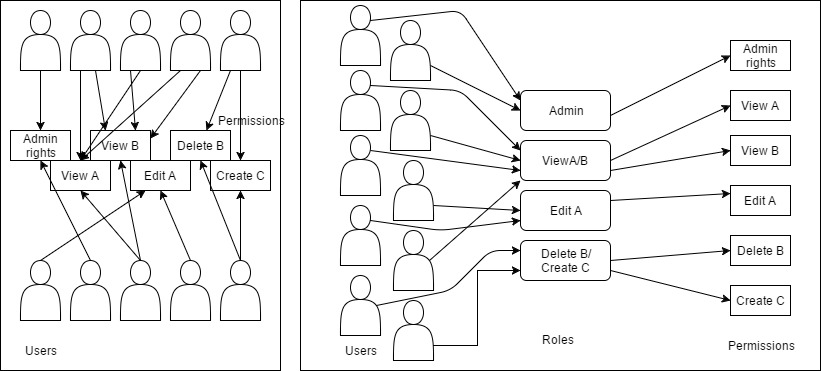
\includegraphics[width=0.9\textwidth, height=0.50\textwidth]{Img/self/RBACvsNonRBAC.jpg}
    \caption{Compares managing users and permissions, left without roles, right with the use of roles.}
\end{figure}
The basic building blocks of the role based access control model are the following (based on the list given in The NIST model for RBAC : Towards a unified standard \cite{Overview1}) :
\begin{itemize}
    \item Each user is assigned to one or more possible roles
    \item Each role gets permissions assigned to them, this number of permissions can vary from none to multiple
    \item A permission is a mapping from an operation to an object
    \item Different roles can have overlapping permissions
    \item Users get the permissions of the roles they belong to, we can use sessions to restrict the active roles a user has at a time and allow them to switch between their different roles
    \item It should be easy to get an overview of users/roles and roles/permissions relations
\end{itemize}
Below is the scheme of the relationship between the different building blocks for the role based access control system. 
We can see that a user can have multiple roles and that roles can be assigned to multiple users as depicted by the double arrow.
The same goes for roles and permission, permissions exist of out combinations between objects and actions.
A user has a single session which in turn can be related to multiple roles, these are the active roles for that user.
In our implementation we limit this to one role in order to maximize conformity with the principle of least privilege. 
This means the user can only access objects with the permissions of one role and not all the other roles they have assigned, but do not need the permissions of at that time, limiting access to the minimal level of accessibility that allows normal functioning of that role. 

\begin{figure}[ht]
    \centering
    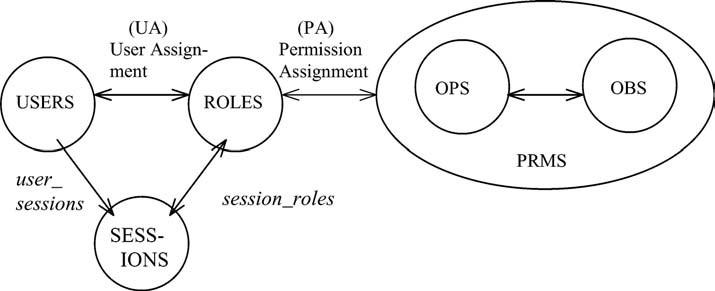
\includegraphics[width=0.7\textwidth, height=0.4\textwidth]{Img/standard/coreRBAC.jpg}
    \caption{Core RBAC scheme, adapted from the NIST standard report\cite{Standard}}
\end{figure}

\subsection{Hierarchical RBAC}
The first extension that can be done on the role based access control model is that of introducing hierarchy.
We give the basics of this extension, for a more in depth view look at the NIST standard\cite{Hierarch},\cite{Standard}.
The idea here is that instead of having multiple individual roles we create a hierarchy of roles.
In this hierarchy a role can get all the permissions from the role it inherits from and have its own permissions assigned to it that the role it inherited from did not have.
While hierarchies can be done in any arbitrary form (general hierarchy), there is also the limited hierarchy which restricts the structure to just trees.
This means that multiple inheritance, a role that derives from multiple other roles, is not allowed for limited hierarchy, but it is for general hierarchy.
Following is the scheme for hierarchical role based access control, it is similar to the normal role based access control one with the addition of a relationship between roles where a role can inherit from multiple roles and a role can be inherited by multiple roles.

\begin{figure}[ht]
    \centering
    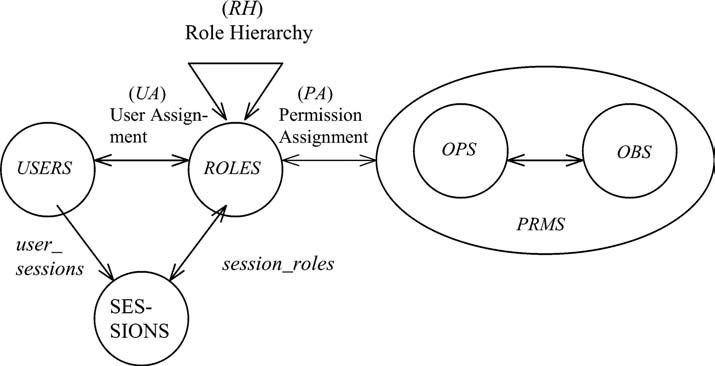
\includegraphics[width=0.7\textwidth, height=0.40\textwidth]{Img/standard/hierarchRBAC.jpg}
    \caption{Hierarchical RBAC scheme, adapted from the NIST standard report\cite{Standard}}
\end{figure}

\textbf{Example} In the image below we can see that we have 4 roles available, User, Employee, Consultant and supervisor. 
All of these roles have their associated permissions A, B, C, D and E.
Since user has the permission A associated with it and all other roles inherit from the User role this means that all other roles also get permission A associated with them.
This means that the supervisor role has permissions A, B, C and D, A inherited from User, B and C inherited from employee and D from its own role. 
The consultant role only has permissions A from inheriting from User and its own permission E.

\begin{figure}[!h]
    \centering
    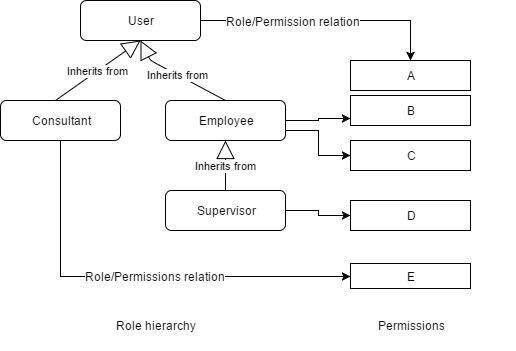
\includegraphics[height=0.55\textwidth,width=0.8\textwidth]{Img/self/ExampleHierarch.jpg}
    \caption{Hierarchical RBAC example}
\end{figure}

\subsection{Constraint based RBAC}
Another extension on the role based access control model makes use of constraints as described in A framework for en-forcing constrained RBAC policies\cite{Constraint}.
Both the constraint and hierarchical extension to role based access control can be used individually on top of the basic model or in combination.
The main idea is that by making use of constraints we can limit human errors made by the administrators that go against rules set by the company.
This also prevents abuse, as well as introduces a way to enforce more specific business rules. 
The biggest reason for using constraints however is to enforce the principle of separation of duty, where we can make it impossible that a single user with all the needed rights can perform a task without the involvement of a second user with the needed rights.
\\
\\
This principle of separation of duty can be enforced in two ways with constraints:

\begin{enumerate}
    \item Static separation of duty, this type of constraint does not depend on any state of an object. 
    
    \textbf{Example} We have 2 specific roles that need to sign off on a task before it can continue.
    With static separation of duty we make it impossible for the manager to assign both of these roles to a single user. 
    This means that we need 2 different users with 2 different roles to sign off on a given task before it can continue.
    
    \item Dynamic separation of duty, this type of constraint depends on the current state of an object.
    
    \textbf{Example} We have a constraint that requires two different people to sign off for a certain action to be done. 
    Even though one person may have all the needed permissions, they can still only do one sign off and someone else with the correct permissions is needed to do the second sign off.
    We look at the state of the system (who has already signed off) to see if a user is allowed to be the second person to sign off.
    
    \textbf{Example} Another example would be the constraint of there may only be 1 CEO at a time, which also depends on the state of the management system.
\end{enumerate}
\\
\\
The image below is the same one as used for hierarchy but now we also have added the blocks Static separation of duty(SSD) and dynamic separation of duty (DSD).
The Static block has a relation with the existing roles in the system and the assignment of roles to users, the dynamic block has a relation with the active sessions to roles relationship.
The dynamic constraints are placed on the sessions and are determined on the current session status.

\begin{figure}[ht]
    \centering
    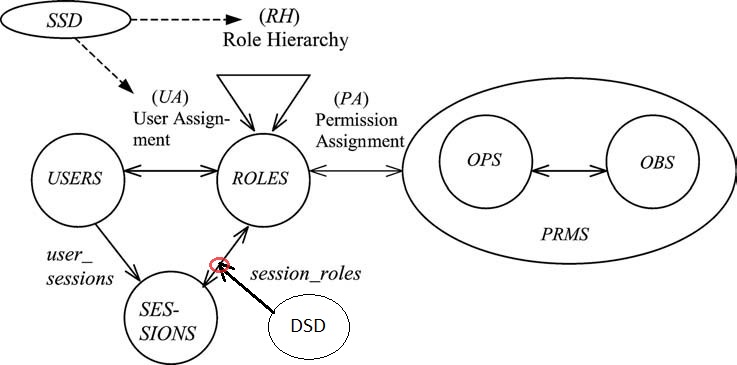
\includegraphics[width=0.7\textwidth, height=0.40\textwidth]{Img/standard/combinedConstraint.jpg}
    \caption{Constrained RBAC scheme, adapted from the NIST Standard \cite{Standard}}
\end{figure}

\section{Attribute based access control (ABAC)}
 Attribute based access control (ABAC) is a more general approach to role based access control. 
 While role based access control only focuses on the user roles, attribute based access control makes use of multiple attributes.
 These attributes can be on users, objects, actions or even environmental.
 By the combination of attributes a user has and the attributes an object has we can decide if that user can access that given object.  
\\
\\
The building blocks for attribute based access control as described in A Unified Attribute-Based Access Control
Model Covering DAC, MAC and RBAC\cite{ABAC2} and Guide to Attribute Based Access Control (ABAC) Definition and Considerations\cite{ABAC} are the following:
\begin{description}
    \item [Attribute]Attributes represent the characteristics of those objects/users/action/environments they are associated with.
    Users, actions and objects can have attributes, apart from this we can also have environmental attributes.
    We can use the value of these attributes to determine if access is granted or not.
    \item [Object] Objects are the things we want to access. Each object has attributes for example when it was created, who created it, what research group it belongs too, etc. 
    \item [User] A user of the system, can be both a machine or human, the user requests access to certain object. Each user also has its own attributes such as the user name, email, date of registration etc.
    \item [Policy] A policy can use the different available attributes from users, objects, the environment and actions to decide on whether or not a user can access a certain resource with that action under those circumstances.
    A policy can be both positive and negative, with negative ones taking priority.
    If you meet a negative policy you are not allowed to perform the action no matter how many positive ones you meet.
    A policy example would be that all users that registered before 1/01/2000 are allowed to access the files created in the 90's.
    \item [Operation] Can be done on an object, these operations can be database CRUD actions as well as execution of functions, actions can also have certain attributes.
    \item [Environmental condition] Do not depend on user and object, this condition is purely dependant on the environment, for example the air pressure in a room or the current time.
\end{description}
\textbf{Example} Using the image below we see that there are 2 users, a senior developer and a normal developer this role is an attribute, both users also have a name as attribute.
There are 3 objects, source code with a critical level attribute, source code with a normal level attribute and a payroll object which has the name of the user it belongs to as an attribute.
3 policies have been defined on the system.
If the user named Al tries to access the payroll his is not allowed since the its the payroll of Bert so only Bert can access it.
Al who is a senior developer can access both the source code of critical and normal level, Bert however being only a developer can only access the source code of normal type.

\begin{figure}[ht]
    \centering
    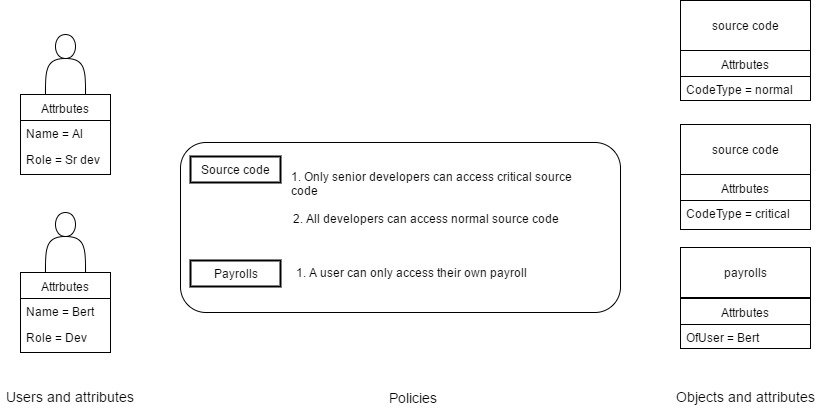
\includegraphics[height=0.45\textwidth, width=0.75\textwidth]{Img/self/ABACExample.jpg}
    \caption{ABAC example}
\end{figure}
The proposed architecture for building  attribute based  access control model as presented in Guide to Attribute Based Access Control (ABAC) Definition and Considerations \cite{ABAC} makes use of the following 4 components:
\begin{description}
    \item [PEP] The policy enforcement point, this point intercepts a call for access and asks the PDP if that user is allowed to access the demanded data.
    If the user is allowed to access it the PEP will let the call pass if not it will refuse it.
    \item [PDP] The policy decision point, this point uses all the data made available to it from a policy database and the different PIP's to make a decision for a user that wants to access certain resources.
    \item [PIP] The policy information point (or points) are databases that provide the attribute information for the different users, objects, actions and the environment to the PDP so it can make its decisions.
    \item [PAP] The policy administration point is used to edit the different policies that exist, this allows a user to add new policies and delete or change existing policies.
\end{description}
The following image illustrates their relationship with each other and the system in a visual way.

\begin{figure}[ht]
    \centering
    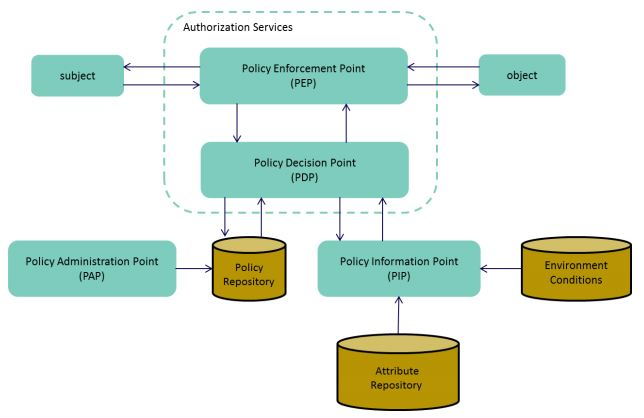
\includegraphics[width=0.75\textwidth, height=0.40\textwidth]{Img/standard/ABACArchi.JPG}
    \caption{Architecture ABAC and relation between the different points, adapted from the NIST Guide to Attribute Based Access Control (ABAC) Definition and Considerations \cite{ABAC}}
\end{figure}

\section{Attribute enhanced RBAC (AERBAC)}
Attribute enhanced role based access control is, as the name suggests, a hybrid form that combines aspects of both role based access control and attribute based access control in a single model in an effort to get the benefits of both models.
These hybrid models can include both the constraints and hierarchy extensions available for RBAC.
This can be done in multiple ways as shown by D. Richard Kuhnet et al in Adding Attributes to Role-Based Access Control\cite{Combined1}, where they sum up the different types of combinations that can be made.
Multiple hybrid versions have been proposed, such as Ting Cai et al their Hybrid attribute based RBAC model\cite{Combined2} where they split up permissions in static and dynamic permissions.
\\
\\
Another such hybrid model, which is the one we focus on, is Qasim Mahmood Rajpoot et al with their Attributes Enhanced Role-Based Access Control Model\cite{Combined3}.
This model enhances the previous handled role based access control model with conditions on the permissions, these conditions make use of different attributes.
This gives the following scheme of the different building blocks and their relationship to each-other.
We can see that on the permissions we can put a set of conditions and that objects and users have attributes related to them. 
For checking access we can also make use of environmental attributes such as current time, temperature and so on.
Using all of these attributes in the conditions we can then evaluate the condition and an allow or deny access decision, that gives access to a resource for a given user, can then be made.

\begin{figure}[ht]
    \centering
    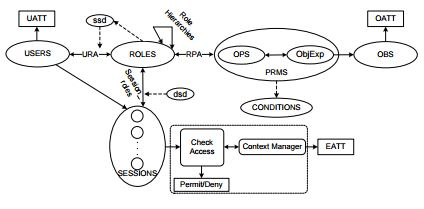
\includegraphics[width=1\textwidth, height=0.45\textwidth]{Img/self/AERBAC.JPG}
    \caption{AERBAC scheme, adapted from Enhanced Role-Based Access Control Model\cite{Combined3}}
\end{figure}
\section{Organizational units}
The idea of organizational units, as defined by M .Umar Aftab et all \cite{OU}, is that apart from only working with roles we will also work with organizational units.
This is an intermediate building block between users and roles which allows us to assign users to organizational units before giving them roles.
Like this users will already be divided on the organizational level, often departments, where already only a sub set of permissions may be applicable, this before they get roles assigned to them.
The permissions are still assigned to the roles.
Doing this allows for a finer grained access control system when dealing with very large multi departmentalized companies.
Below is an example of how the organization would look like when using permissions, roles, users and organizational units.

\begin{figure}[h]
    \centering
    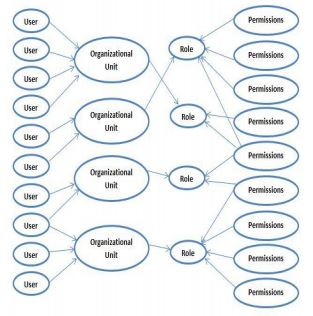
\includegraphics[width=0.75\textwidth, height=0.55\textwidth]{Img/self/OUExample.JPG}
    \caption{Overview of management using organisational units, adapted from RBAC Architecture Design Issues in Institutions Collaborative Environment \cite{OU}}
\end{figure}

\clearpage
\section{Task role based accesss control}
Task role based access control as described by Seog Park Sejong Oh in Task-role based access control models\cite{TBRC} is an access control model that builds further upon role based access control with the hierarchy extension.
This hierarchy is not the one described earlier, but it is a supervision role hierarchy model.
This supervision role hierarchy resembles the hierarchy in role based access control, the key difference being that a derived role does not have to inherit every permission of the roles they are derived from. 
In task role based access control permissions are first assigned to tasks and later on these tasks are assigned to roles. 
Tasks are focused on the activities that need to be done while roles are focused on the users.
Task role based access control is mostly used when managing work flows.
\\
\\
Tasks have three attributes that play a role in task role based access control:
\begin{description}
    \item [Activation condition] The condition that has to be met to activate a task, making it possible to activate/execute that task.
    \item [Time constraint] How long a task remains active after it has been activated.
    \item [Cardinality] The number of instances of a specific task that can happen at a time.
\end{description}

 When we make use of an activation condition we call this active access control. 
 If a person has permissions to do a task but it is not active then that person cannot do it.
 Passive access control is how it is done in normal role based access control, a person gets permission so they can access the resource, this can also be done in task role based access control.
 The time constraint is linked to this as it controls how long a task is activated and can be accessed before becoming inactive again.
 Cardinality controls how many users can complete a task at the same time while the task is active.
 \\
 \\
The scheme below is the same as the one used for the other models, the difference being that the hierarchy on roles is now the supervision role hierarchy. 
Also tasks are introduced that are associated with  the different roles instead of permissions, permissions are now associated with the tasks.
This is only the set of permissions that fall under the activation condition of the task, if we work with such a condition.  
Those permissions that do not fall under this activation condition are not valid for the task at that time.

\begin{figure}[ht]
    \centering
    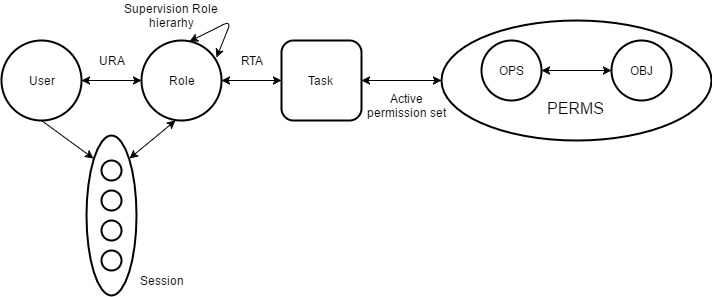
\includegraphics[width=0.7\textwidth, height=0.39\textwidth]{Img/self/TBAC.jpg}
    \caption{TBAC scheme partially adapted from Task-Role Based Dual System Access Control Model\cite{TBAC2}}
\end{figure}


\section{Prototype choices}
The choice of prototypes is primarily steered by the requirements put forward by the system we use as a case study.
The most straightforward choice was to prototype the role based model and the attribute based model as these 2 approaches stand out as most interesting.
However due to the requirements of the application that is being studied, which we  explain in depth in the next chapter, we need a model that allows more fine grained access control.
\\
\\
First of all we implement the attribute enhanced role based access control model.
This model starts from the role based access control model but adds fine grained access control that the original model lacks and that is required for the application being studied.
This is done by adding attributes to the permissions.
Roles hold a special status over the other attributes, where roles have the permissions assigned to them.
These permissions can have conditions associated with them, which use the other attributes.
This model can be extended the same way as role based access control, with hierarchy and constraints, we did not implement this.
\\
\\
The second model we implement is the attribute based access control model, this is a more general approach that does not rely on roles to be associated with rules. 
Instead the policies made are enforced on the complete system, every time someone tries to access an object all rules on that object will be tested.
There will still be roles, but they are one of the attributes that is being used in this model, they are just part of the conditions that are being used.
\\
The role based access control model is not implemented because the basic requirements for the case study we perform require more fine grained access control than role based access control offers.
However the basis of this model is part of the implementation of the attribute enhanced role based access control model.
It is possible to let this model behave as the role based access control model by not using conditions.
We will not prototype organizational units because this approach is mainly to make management easier, which can also be done with other methods which expand on what we already have as a system.
The task role based access control model will also not be prototyped since the added possibilities and complexity are overkill compared to the needs of the project.
All of these models excluded can be part of future work on the subject.
\chapter{Case study}
\label{chapt:Case study}

In this chapter we go over what it is exactly we did in the case study.
We go over the requirements of the system and how that influenced the choice we made in the previous chapter on which model to implement and research.
Apart from the target system we also discuss the technology used and how we build up the different models, their architectures and where the big differences between the models can be found.

\section{Target system: BESC}
The target system for our case study  is the BESC application developed by 4DVision\footnote{\url{http://www.4dvision.be/}}. 
This is a system used for importing and exporting cargo in or out of Congo.
The system consists of exporters and forwarders which are associated with a company and which need to make a visa request for importing/exporting goods.
These visa requests then have to be approved by the agents assigned to that forwarder/exporter. 
These agents can approve only a certain number of requests depending on the visa points they have available, they can also request corrections on visa requests or refuse the visa requests.
In general agents are assigned to exporters and forwarders depending on the country from which they operate and their language.
Between agents there is a hierarchy with national/global/control agents that do supervision and provide additional visa points.
\\
\\
This system's access control is currently done by statically checking if given roles are allowed to access certain objects, putting the role checks in the code. 
With our models we provide a more dynamic approach to access control, this means that we can change the access control rules while the system is running.
An admin can then configure the different models depending on the needs, this means no new development is required when the access control needs change.
Apart from this requirement of dynamic access control the models should be able to meet following requirements that are in the original BESC system:
\\
\begin{enumerate}
    \item Objects can only be accessed if a rule has been made for the objects, if no rule exists nobody has access. Only those users conforming to the rule can access it. This includes rules saying everyone has access to that object.
    \item Only users that are logged in can be granted access, all others are denied by default.
    \item Get, Put, Post and delete should be supported.
    \item It should be possible to add custom actions that have access rights attached to them.
    \item It must be possible to only be able to access objects when one of their fields has a certain value.
    \item It must be possible to hide certain objects their fields if no access to that field is granted. The user should not even know the existence of the fields.
\end{enumerate}
\\
With the last two requirements it becomes clear that there is a need for fine grained access control where we can deny access depending on the values of certain fields (which will be our attributes) or deny access to these fields as a whole.
The role based access control model as described in the previous chapter does not allow for this kind of fine grained access control, meaning that another model has to be decided on.
Attribute based access control meets these requirements and this is due to the introduction of attributes.
Given these two observations we look for models that are a hybrid version of the two models.
We need a hybrid that combines the concepts of role based access control and introduces the concept off attributes and conditions from attribute based access control to allow for fine grained access.
We find these needs fulfilled using the attribute enhanced role based access control model, which is the model we use instead of the role based access control model.

\section{Approach}
There are two main options for adding access control models into this application.
The first option is to use existing frameworks that have already implemented these models, the second option is to implement these models into the BESC application ourselves.
Both these approaches have their positives and negatives which have to be taken into consideration before choosing which approach we take.
\\
\\
The positive points of the first option are that in this case we already have a working solution that is less likely to contain errors and a solution that has a tried and tested user interface adapted to the needs of using the models properly. 
The downsides however are that because attribute enhanced role based access control is rather novel there are no out of the box solutions for it yet, meaning we would have to create this ourselves.
For attribute based access control the implementations that are available are generally not open source and those that are are not mature enough yet.
This would also require us to learn how to setup the different systems and how they can be applied to the existing application that we test.
\\
\\
For option two the positives are that when implementing these models ourselves we can control the environment properly and implement the models in a similar way.
This to make sure that the differences and problems noticed are caused by the nature of the models and not because the solution provided for one model is better developed or uses better technology than the solutions that are available for the other model.
The downsides are that by developing this ourselves we are limited to what we can create ourselves, we wont be able to reach the quality of out of the box solutions with years of development that have a high quality user interfaces while we are working on this with limited time and resources.
Some scoping has to be done here which we have to take into account when doing the study,making sure that the metrics gathered and questions asked research what is in the scope of our study, we discuss this further in the next chapter. 
We are also required to go in depth into the architecture of the existing application in order to integrate our security models into it.
This also requires learning a new language and using a new environment since the original application has been build using C\# in the .net core framework, with which we have no prior experience.
\clearpage
We have chosen to go with option two, since there are no existing implementations yet for attribute enhanced role based access control that are available we have to provide this ourselves either way. 
Because of this we already have to overcome most downsides of approach two even if we were to choose an existing implementation of the attribute based model, this makes it logical to also implement the attribute based model ourselves.
Doing so ensures that the models have the same grounds of comparison, use the same technologies and have the same abilities if it comes to creating rules.
This also gives us optimal flexibility when we need to adapt the systems to our needs as stated in the requirements.

\section{Technology and implementation}
As mentioned before the BESC application is written in C\# and makes use of the .net core framework, we also implement our models using this language and framework.
Different components are needed, we divide the models in 3 different parts:
\begin{enumerate}
    \item The management component, this component is made for the management of users, their roles, adding permissions and attaching them to roles in the attribute enhanced role based model and adding policies for the attribute based model, including their conditions. 
    This allows for adding and removing each of these entities to the system (except users which is already available in BESC) and setting up the relationships between them.
    \item The access control component, this is the component that upon receiving a request for access gets all the policies/permissions involved and makes use of the evaluation component to determine if access is allowed. 
    This is the component that checks if the rules are positive or negative depending on the result of the evaluation of the conditions.
    It also keeps track of fields that have been hidden and takes the appropriate steps to make sure they do not get passed to the front of the application.
    It is also this component that is responsible to add the needed queries when partial access is allowed.
    \item The evaluation component, this component evaluates the different conditions put on the policies/permissions and checks if a condition is met or not, which is used by the access control component to make a decision on allowing access or not.
\end{enumerate}


\subsection{Management component}
In this section we go over the management component implemented in BESC, this for both models.

\subsubsection{Attribute enhanced role based access control}
The image below shows the database scheme of the structure of managing the system, this resembles most architectures used for role based access control:
\\
\begin{figure}[h]
    \centering
    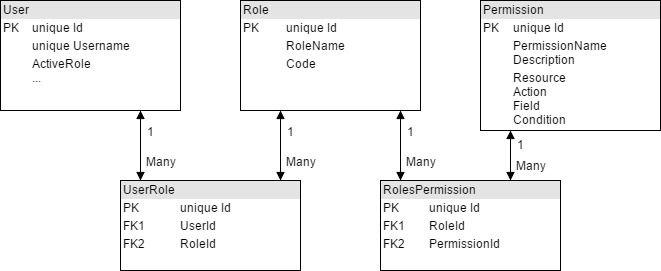
\includegraphics[width=0.7\textwidth]{Img/self/RBACManagementDiagram.jpg}
    \caption{Database diagram for AERBAC management}
\end{figure}
\\
We see that we have users with some fields, username Id etc but most importantly their active role. Since the system allows for users to have more roles and being able to switch between those roles we use this field to keep track of the user his current role.
Then we have the role objects in the system which have a code and name, all that is needed for a role to be identified in a system.
The third important part is the permission, it has multiple fields with the most important ones being Action, Resource, Condition and Field. 
The action represents what action can be done on the objects of type resource, possibly with a certain condition that allows viewing a specific field of that object.
These last two are optional.
Apart from these three we have some helper tables to allow for our many to many relationships where multiple users can be associated with multiple roles and multiple roles can be associated with multiple permissions.
The attribute enhanced aspect of the model is primarily contained in the Condition and Field attribute fields of the permissions.
\\
\\
Another part of the management component is the user interface, the user interface is used for the admin of the system to add new roles, assign these to users, add permissions and assign these to roles.
In our case study we have made a very basic user interface to allow these functions .
Below you can see how permissions are added to the system as well as how we add roles and assign them to users and assign permissions to roles.

\begin{figure}[h]
    \centering
    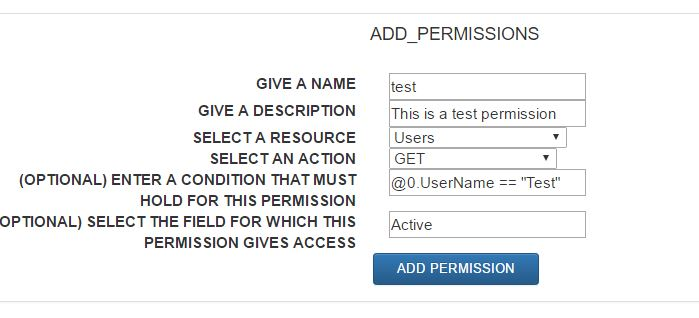
\includegraphics[width=0.7\textwidth, height=0.22\textwidth]{Img/Tool/AddPermission.JPG}
    \caption{Adding permissions in AERBAC}
\end{figure}
\begin{figure}[h]
    \centering
    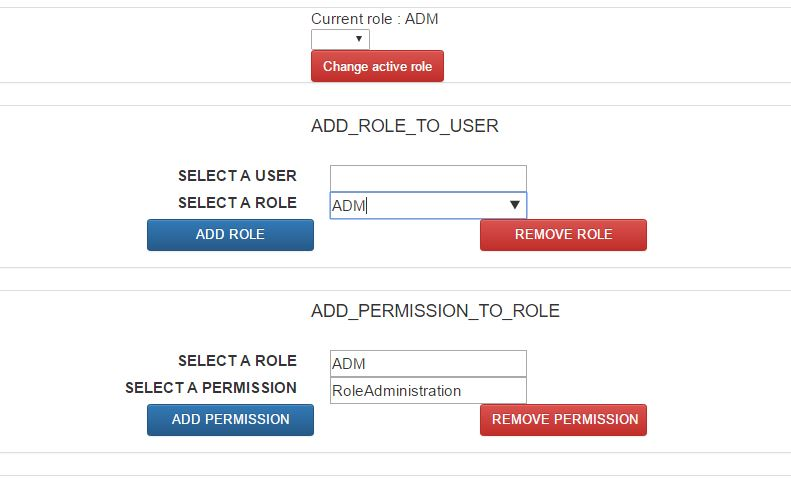
\includegraphics[width=0.8\textwidth, height=0.45\textwidth]{Img/Tool/RBAC_AddRP.JPG}
    \caption{Adding roles and permissions and changing roles in AERBAC}
\end{figure}

\subsubsection{Attribute based access control}
The image below (3.4) shows the database scheme of the structure of managing the system using the attribute based access control model:
\begin{figure}[h]
    \centering
    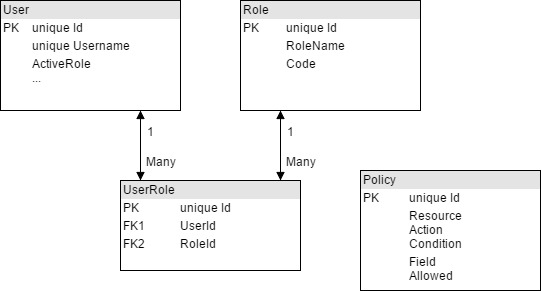
\includegraphics[width=0.7\textwidth]{Img/self/ABACManagementDiagram.jpg}
    \caption{Database diagram for ABAC management}
\end{figure}
\\
\\
Just like in the previous model we have users and roles, the only reason however that we have roles like this is because we want the system to support having multiple roles on a single user, this model could just as well do without the roles.
Unlike the previous model roles are not first class citizens here over the other objects and their attributes.
Once again we also have a helper table for the relationship between users and roles.
Instead of permissions however we now work with policies, these policies have no relationship with any of the other parts.
The important fields in these policies are Action, Resource, Condition, Field and Allowed. 
Again these mean practically the same as with the previous model, except that now a condition is not optional and should always be provided and the allowed field, which allows for setting both positive and negative policies.
The negative policies are stronger than the positive ones and if the condition on these negative policies is met then access is denied completely.
\\
\\
Once again a very basic user interface for the admin of the system, in the attribute based model the admin can add roles, assign users to roles and add policies to the system.
The interface is specifically kept as close as possible to the previous one in order to try and minimize the effects of the user interface on using both models.
Below you can see how policies are added to the system as well as how the UI looks like for adding roles and assigning them to users and for users to change their active roles.

\begin{figure}[h]
    \centering
    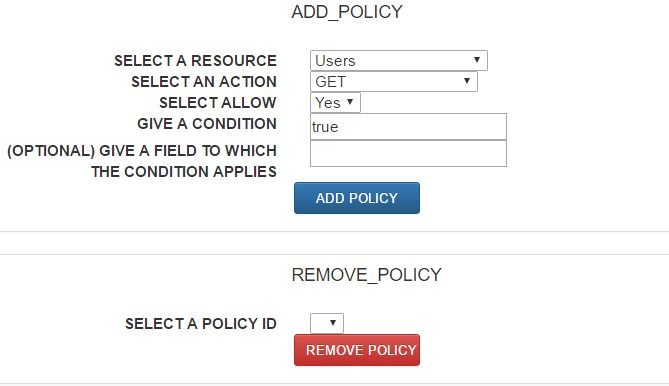
\includegraphics[width=0.7\textwidth]{Img/Tool/AddPolicies.JPG}
    \caption{Adding policies in ABAC}
\end{figure}
\clearpage
\begin{figure}[h]
    \centering
    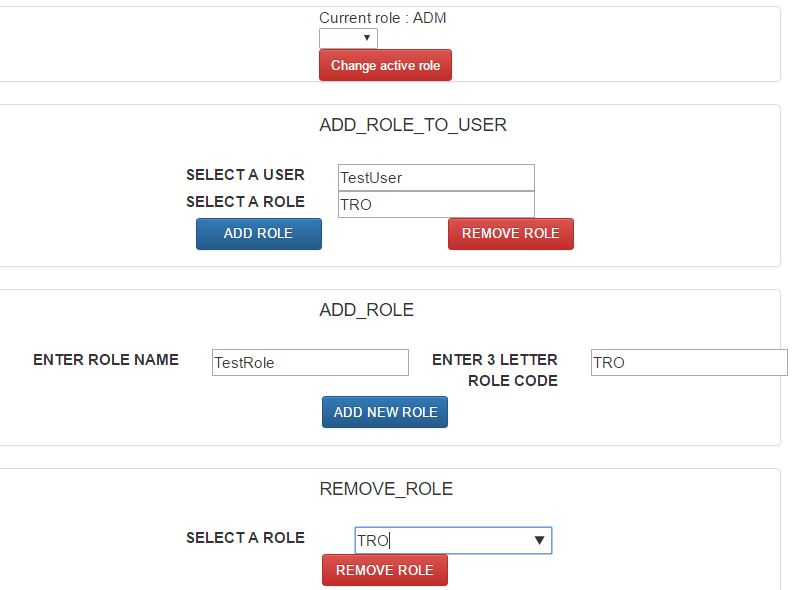
\includegraphics[width=0.7\textwidth]{Img/Tool/ABACADD.JPG}
    \caption{Adding and assigning roles in ABAC}
\end{figure}

\subsection{Access control component}

We implemented the  access control component in 2 layers, first we have a layer that checks if a user can do the requested action on the type of object, without looking at values of the attributes of the different objects.
Doing this prevents  that we already have to access the objects and do conditional checks if we are not supposed to access those objects at all, independent of the values of the attributes.
This is to prevent unnecessary computations taking up extra time.
The second layer is when conditions have to be applied to specific objects and the user can only do something with a subset of that object type.

\subsubsection{Attribute enhanced role based access control}
In the case of attribute enhanced role based access control we have 3 different cases:
\begin{itemize}
    \item There is no condition on the permission at all.
    \item The conditions only contain attributes that are not part of the object we want to access, such as user data.
    \item The conditions contains attributes of the object we want access to.
\end{itemize}
\\
In case one and two we can do the evaluation in layer one, we do not need specific object data to evaluate these conditions.
In case three we already need to be able to access the object before the condition can be evaluate, if there was already a negative response in the previous layer this will not be executed.
When using the fields option, which allows for hiding certain attributes from the users, the permission only counts for the field in question on that object, not general access to the object.
Once such a permission is made the field is invisible for everyone who does not meet this permissions condition.
This functionality is also part of the second layer.


\subsubsection{Attribute based access control}
In the case of attribute based access control we have only 2 cases since we must always have a condition on the policies:
\begin{itemize}
    \item The conditions only contain attributes that are not part of the object we want to access, such as user data, this includes conditions that just contain true.
    \item The conditions contains attributes of the object we want access to.
\end{itemize}
\\
Analogous to the previous model we have that the first case is checked in the first layer, the second case is checked in the second layer if we get there.
\\
\\
When using the fields option, which allows for hiding certain attributes on the objects from the users, when a policy is set for hiding a field then everyone who does not meet the policy cannot see the field.
This policy however only affects the fields, it does not deny or grant access to the object as a whole another policy has to be made for that.
Again this functionality is also a part of the second layer.
\\
\\
Another specificity with the attribute based model is that we have the option of negative policies.
The negative policies are always evaluated first and are the strongest policies, if the condition of a negative policy is met this means there is no access allowed at all.

\subsection{Evaluation component}
This component is a component that is used in both models in the same way.
Building this component mainly relies on the use of the dynamic LINQ library\footnote{\url{https://github.com/StefH/System.Linq.Dynamic.Core}}.
This is an extension to the linq (language integrated query) functionality that is part of the .net framework, this lets us use a query syntax in the code, which allows queries to be generated from code with similar syntax.
Dynamic linq allows to apply the query capabilities linq provides by using and evaluating strings while the system is running.
Depending on the difficulty of the queries this is evaluated either on database level or on code level (or both).
Doing this allows for a language that the participants in our study are familiar with since it resembles the capabilities of the programming language they are used to.
\\
Below is an example of the conditions we have, this is for the attribute based model:
\begin{algorithm}
    (Code == "FWD") and @0.ActiveRole == "ADM"
\end{algorithm}
\\
This is a piece of code to access the roles that are available in the system, this condition checks if the Code field of the role object we want to access has the value "FWD" and if the current user has as its active role "ADM".
We can see a few different features of using dynamic linq here that make it useful for using as the core part of our evaluation component:
\begin{itemize}
    \item Access to the fields of the object you are working on just by using their field names (the Role object has a field Code). The fields can also be chained just like while programming to get objects that can be part of that object using the . operator.
    \item Availability of boolean operators and, or, not as well as the use of ( and ) to form boolean expressions.
    \item Can input constant strings with "" and other constants just as in normal programming.
    \item Availability of placeholders that can be put into the conditions that can make use of attributes of other objects if needed. This is generally done to get external attributes into the system. In the example we can see this is done by using @ and then the number of the object that is available. In the case of the example we have @0 which is where the object of the user making the request is contained and then the field of that object, its ActiveRole.
\end{itemize}

\chapter{Experiment}
\label{chapt:Experiment}
In the previous chapters we went over the different models that were available in literature, the models we have chosen to implement and compare, the requirements for these models and how they were implemented.
In this chapter we explain our experiment, what exactly is our experiment, what do we want to accomplish with it, which are the variables that are at play in the experiment, what metrics/data do we gather and why do we gather those metrics/data.
The results of the experiment are presented and reasoned about in the next chapter.

\section{Experiment goals}
The goal of the experiment is to find out on different levels which model performs better in the hands of users that will manage the system with both these models.
These users can either be system administrators within the company or the developers of the system.
We look at the manageability of the models for the administrators, which one is the easier one to manage, less error prone, fastest.
We also look at the performance of the different models, abilities that the different models have concerning their features and how this affects the usability of both models.
We hold an interview with the users so we can also get their experiences with the different models and what they thought about them. 


\section{Experimental setup}
To prepare our users for managing the system with the different models we first give them a small introduction on how to use the different models.
This introduction includes showing the functionality of the different models, explaining specific behaviour such as how the hiding of attribute fields works and behaves and also how negative policies have priority over normal ones, the examples shown are representative to the tasks the users have to perform.
Because of the minimal user interface we provided it is needed to give the users some extra information about the system, this is provided to them by means of a cheat sheet on which we give them the following extra information:
\begin{itemize}
    \item The attributes available on the different objects.
    \item The included external sources of data and their corresponding placeholder.
    \item Id to string mappings which are needed to know the status of some objects.
    \item Short summary of what was told in the introduction.
\end{itemize}
\\
The \textbf{users} are given multiple \textbf{scenario's} which each of them has to complete using the available \textbf{access control models}.
These are the three variables that varied during the experiment, there are two different scenario's, two different users and two different models which makes for a total of eight experiments that are being conducted.

\subsection{Users}
There are a total of 2 users that take part in this experiment, these users have varied experience with the BESC system that already existed before implementing the access control models.
One of the users is an advanced user that has significant knowledge of the inner workings of the BESC system as well as the systems underlying data model.
This while the other user has not been involved with the development of the original system and has no extra knowledge about the BESC system aside from what we have provided on the cheat sheet.
We have chosen for this difference in knowledge about the system to be able to compare the needed knowledge that is needed to manage the different models and whether or not having minimal knowledge about the system has a negative effect on the results. 

\subsection{Scenario's}
As our scenario's we have chosen two parts of the functionality that is offered in the BESC system.
These scenario's have been chosen to showcase the two big requirements put forward by the system on fine grained access control, namely only accessing objects with certain attribute values and hiding certain attributes as a whole for the users.
The first scenario is longer in number of tasks that have to be taken by the managing user and is a scenario where limited knowledge is needed, mainly meeting the first requirement stated.
The second scenario is shorter in the number of tasks that have to be done by the users but the tasks are more complicated, require more knowledge of the system and showcases the second requirement for fine grained access.
Both of these scenario's can be found in the appendix \ref{appendix:scenario} of this thesis.

\subsection{Models}
These are the attribute enhanced role based access control model and the attribute based access control model we have implemented into the BESC application.

\section{Data capture}
In this section we give an outline of the different metrics that are looked at to evaluate the models of access control that we implemented.
An explanation is given of what we mean with each metric and how we measure/evaluate this metric.
\subsection{Chosen metrics}
Following are the metrics we wish to measure and research, we explain for each of these metrics what we mean with them.

\begin{description}
    \item [Manageability] Under manageability  we  look  at  how  easy  it  is to  manage the system for the admin, it is a broader term for multiple metrics.
    This includes the correctness in managing the system using both models as well as the maintainability.
    We also look at the speed of setting up the access control with both models and the number of rules needed to set it up.
    We also look at the experiences the users had with each model.
    \item [Correctness]  Correctness is seen as the amount of mistakes made by the users managing the system which lead to access to objects that violated the requirements.
    \item [Maintainability] Maintainability deals with how easy it is to manage the existing system once the requirements on access control change or a new person is put in charge.
    \item [Understandability] With understandability  we  look  at  how  easy or difficult it is to understand for users what they are allowed to access.
    We also look at the admins and how easy it is for them to analyze the system with the different models and  and find out who has what access rights.
    \item [Extensibility] With extensibility  we want to know if the models could easily be extended with new features and which features that would be.
    \item [Performance] With performance we mean what effects the use of the different models has on the time to get access to an object. 
    The computation time it takes to evaluate if a user has access or not.
\end{description}

\subsection{Capture methods}
In this section we explain how we test for the different metrics explained in the previous section.
We have 3 ways in which we obtain this data:

\begin{enumerate}
    \item The case study itself where we measure the performance of the users.
    \item A concluding interview with the users where we wish to measure their experiences with the different models, the interview questions can be found in appendix \ref{appendix:interview}.
    \item A performance test where we test which system does the access evaluation the quickest and in which circumstances.
\end{enumerate}
\\
For each of the metrics we mention which of the above methods gave us the data for it.

\subsubsection{Manageability}
This part is done by doing an in depth interview with the participants of our experiment as well as data gathered from the experiment itself.
There are multiple aspects to this part, the bigger ones are maintainability and correctness which are explained on their own below.
The smaller aspects to this are:
\begin{itemize}
    \item The system setup time, how long it takes for the system to be set up in the different models given the requirements in the scenario's.
    This is measured by timing the users in the experiment.
    The order in which the experiment is done is first scenario one in the enhanced role based access control model, after that scenario one with the attribute based model, then the same order for the second scenario.
    This so that we had sufficient time to do the manual tests for correctness (we had 1 environment for each model).
    \item The number of rules that was used with each model, this was also measured from the experiment.
    For this we simply look at how many permissions/policies were needed to put to get the working system.
    We also take a look at the complexity of the rules.
\end{itemize}

\subsubsection{Correctness}
With correctness we measure the number of mistakes made by the persons managing the system with the different models, this data is gathered from the case study itself.
After the users set up the rules using the different models we manually try to get access to those parts of the system to see if we have access when we should have it.
We also try to get access to parts we should not have access to, this to check if we can really not access them.
We notice there are 3 types of errors that happen:
\begin{enumerate}
    \item Syntax errors are errors that happen because the users are mistaken in the syntax used in the conditions.
    The usual mistakes here are putting a single = instead of == for comparisons or exchanging @ with \$ as a placeholder.
    Since these mistakes have nothing to do with the models themselves but are all about syntax we exclude these errors from the study, these are corrected before we test the number of errors made.
    \item Logical errors are the second type of errors that can happen.
    These logical errors are made in the conditions and lead to the results being different than what was required.
    Evaluating the conditions still succeeds but the result does not meet the the requirements.
    The system still keeps evaluating the other rules.
    The usual mistakes here are bad use of and/or operators or working with a wrong attribute on an object, but the used attribute does exist.
    We measure this error for correctness.
    \item Bad attribute errors, these errors happen when we try to access attributes that an object does not have in the conditions on that object.
    These errors result in the system giving an error, not further evaluating the other rules that should still be checked, but instead just not allowing any access.
    We measure this error for correctness.
\end{enumerate}

\subsubsection{Maintainability}
The data for maintainability is mainly gathered from doing the interview that is provided in appendix \ref{appendix:interview}.
We ask the users for their view on the aspects of how easy it would be to be make changes or be put in charge of the system, we want to find out from the users if they experience a difference between the two models.
The interview contains multiple questions aimed at getting an answer on the maintainability of the system with the different models.
\\
\\
We ask the views of the users for acting as existing admins when policies/permissions are added to the system with the following question:
\\

\textbf{\say{How clear were the interactions between existing policies/permissions and the newly added ones? Was it always clear what the effects of the additions were?} }
\\
\\
We also try to get insights in how easy the admins think it would be for a new admin to work with the existing system by asking hem the following:
\\

\textbf{\say{Looking at the permissions and policies, how easy to understand would it be if you were put there as a new administrator for the system?} }
\\
\\
Lastly we want to know how the users expect the maintainability of the system to be once it starts scaling up, what is the scalability of maintenance. For this we ask following question:
\\

\textbf{\say{Do you foresee any problems that can arise from using these models in systems that are bigger?} }
\\
\\
While these are the main questions with maintainability in mind we can also go into this with the more general questions on which model they prefer over the other and for what reasons this is.
\\
\subsubsection{Understandability}
Understanding what a user can do is critical, both for the admins of the system as for the users themselves.
In our interview we ask our users which of the models is easier to understand, why this is the case, what would be needed to improve this and which model they find the best suited (from a developers standpoint) to make the access rights of users clear to them.
Some of the questions for this goal overlap with manageability.
\\
\\
We ask for the difficulty of understanding the access rights for new admins to the system, using the different models:
\\

\textbf{\say{Looking at the permissions and policies, how easy to understand would it be if you were put there as a new administrator for the system? Is one model better suited to do this than the other?} }
\\
\\
\\
We are also interested in their views as a developer on which model is best suited to make an interface more elaborate than the basic one we provided, in order to make it clear for the users what they are allowed to do:
\\

\textbf{\say{ Looking at it as a developer,  which model would be best to make the users easily understand their access rights?  Why do you think this is the case?} }
\\
\subsubsection{Extensibility}
For extensibility we mainly look if both models provide the features needed to meet the requirements of the system we have established in chapter three.
We also want to get an insight into what features the users would like to see in the models and whether or not some extensions seen in chapter two would be considered useful.
We extract this information trough our interview.
\\
\\
First of all we ask if the users were able to complete the scenario's in both models with the provided features:
\\

\textbf{\say{Were you able to complete all requested actions in the scenario,  given the available feature set?} }
\\
\\
We also ask the users to name other features they would see as being useful as well as put forward an idea of our own (role hierarchy) with the following question:
\\

\textbf{\say{Are there any features that you think would benefit the different models?  What benefits do they provide?  Example of possible features:  role hierarchy.} }
\\
\subsubsection{Performance}
With performance we measure response times between the different models. 
The main goal here is to compare and see if there is a meaningful difference in the response times  between the attribute enhanced roles based model and the attribute based model.
To do this we set up the system with the needed rules in place for 3 users with different roles, this this setup coincides with the first scenario given in appendix \ref{appendix:scenario}.
We then do 100 requests for 100 objects, with a 100 seconds between the calls for each of these models.
We measure the time it takes to receive the call and check it those 100 objects confirm with the rules that are put on the system, we also check if the call was successful or if an error happened.
This data is gathered using the performance test.
\\
\\
Since performance is predominantly tied with the evaluation of the different conditions we also asked the test admins to to their preferences concerning conditions in our interview.
\\
\\
We ask them for their preferences on complex/simple conditions with following question:
\\

\textbf{\say{When using conditions did you prefer adding 1 permission/policy with complex conditions or multiple permissions/policies with simple conditions?} }
\\
\\
We also want to know if they have other ideas for expanding what conditions could do:
\\

\textbf{\say{What do you think about the options that are available for constructing conditions?  Would they suffice for the systems you develop?  If not what additions could be made?} }

\chapter{Results}
\label{chapt:Results}
In this chapter we present the gathered date from the experiment described in the previous chapter.
We provide the data gathered from the interview with the participants and the result metrics from executing the different scenario's as well as the data from the performance tests.
Given this data we formulate our conclusions as to which model performs better in which cases. 
When there are threats to the validity of the data we will also try and deal with those when presenting the results for the data.
\section{Results metrics case study}
These are the results of the management experiment where we let two users manage the system for access control. 
We have four cases for each scenario that had to be managed:

\begin{itemize}
    \item Case 1: User 1 with the attribute enhanced role based model
    \item Case 2: User 1 with the attribute based model
    \item Case 3: User 2 with the attribute enhanced role based model
    \item Case 4: User 1 with the attribute based model
\end{itemize}
\clearpage
\subsection{Setup time}

\subsubsection{Data}

\begin{table}[h]
    \begin{tabular}{ |{2cm}|p{2.5cm}|p{2.5cm}|p{2.5cm}|p{2.5cm}|  }
        \hline
        \multicolumn{5}{|c|}{Timing of managing scenarios} \\
        \hline
        Scenario & case 1 & case 2 & case 3  &case 4\\
        \hline
        1 & 58 min    & 26 min    & 40 min    & 18 min\\
        2 & 41 min    & 32 min    & 32 min    & 23 min\\
        \hline
    \end{tabular}
    \caption{Table results timing}
\end{table}

\subsubsection{Conclusion}
Looking at the data we could conclude that the setup time for the attribute based model is at all times lower than the setup time for the attribute enhanced role based model.
However looking at the experiment we did we can see some problems that lead to these results, first of all the order in which the tests were executed.
Since we let them do each scenario with the attribute enhanced role based model first this took more time due to the nature of the scenario, this caused habituation towards the scenario leading to better timings with the attribute based model.
Another factor influencing these results came to light during the interview,  the users pointed out that the user interface for the attribute based model allowed them to add policies much faster than they could add permissions.
\\
\\
Another trend we notice is that the advanced user took most advantage on setup time of using the attribute based model over the attribute enhanced role based model.
This is because this user made more use of negative policies in the attribute based model, since this user already knew most of the specifications of the system it was possible to use that knowledge to work more efficiently with the negative policies.
\\
\\
We can see a pattern with the data that has been gathered, which clearly favours the use of the attribute based model for both users with a bigger gain for the more knowledgeable user on the level of the setup time.
However there are certain issues with the experiment that do not allow us to make this a definitive conclusion, another experiment where we keep in mind the habituation to scenarios and use more model appropriate user interfaces should be done to either confirm or refute these results.
\clearpage

\subsection{Number of rules}
\subsubsection{Data}

\begin{table}[h]
    \begin{tabular}{ |{2cm}|p{2.5cm}|p{2.5cm}|p{2.5cm}|p{2.5cm}|  }
        \hline
        \multicolumn{5}{|c|}{Number of rules used in management scenarios} \\
        \hline
        Scenario & case 1 & case 2 & case 3  &case 4\\
        \hline
        1 & 44    & 45    & 45    & 61\\
        2 & 23    & 28    & 26    & 32\\
        \hline
    \end{tabular}
    \caption{Table results number of rules}
\end{table}

\subsubsection{Conclusion}

From the data we see that the attribute enhanced role based model consistently results in less permissions compared to the number of policies in the attribute based model, even if only marginally in some cases.
We can also see that for the more advanced user this difference is smaller than for the inexperienced user, this because having more and better knowledge of the system allowed this user to make better use of the negative policies option provided by the attribute based model.
\\
\\
We also noticed that the advanced user preferred putting many conditions together while the inexperienced user chose for using small conditions that were easy to understand, leading to more policies in the attribute based model.
This led too a big difference because we could reuse permissions from the attribute enhanced role based model, but once a policy was made with a specific role in mind another policy had to be made for every other role even if they had had the same access rights, which is what the inexperienced user did.
\\
\\
Lastly there is also a discrepancy between the scenario's, for the more difficult but shorter scenario (scenario two) we notice that the experienced user also needs more policies in the attribute based model compared to when using the attribute enhanced role based model. 
\\
\\
The pattern here shows that the attribute enhanced role based model consistently performs better, especially for the inexperienced users.
The benefit of using this model for the number of permissions is also clearly seen when working with more complex scenarios.
The model also allows for reuse of permissions with different roles without adapting them, making it easier to work with.

\clearpage


\subsection{Correctness}

\subsubsection{Data}
\begin{table}[ht]
    \begin{tabular}{ |{2cm}|p{2.5cm}|p{2.5cm}|p{2.5cm}|p{2.5cm}|  }
        \hline
        \multicolumn{5}{|c|}{Correctness of management scenarios} \\
        \hline
        Scenario & case 1 & case 2 & case 3  &case 4\\
        \hline
        1 & 2 errors    & 4 errors    & 2 errors    & 3 errors\\
        2 & 6 errors    & 7 errors    & 6 errors    & 7 errors\\
        \hline
    \end{tabular}
    \caption{Table results correctness}
\end{table}


\subsubsection{Conclusion}

We can see that using attribute based model consistently produced more errors than using the attribute enhanced role based model.
Analyzing the type of errors we notice that these are very similar in both models but that the effects of the errors, when using the attribute based model, are greater.
Just making logical errors has the same effect using both models, however making attribute based errors causes the system to give errors, which fails in every case that policy/permission is used.
Since the attribute based model runs all policies for a given object all access attempts to that object fail since they all have to evaluate that policy. 
With the attribute enhanced role based model on the other hand this effect only happens when that permission is assigned to a given role, not giving an error when the other roles want to access the object.
\\
\\
In the case where errors are being made, which should be limited in order for both models to properly fulfill their tasks, the attribute enhanced role based model is the better choice since it limits the area where the error can lead to faults in the system.

\section{Results interview}
In this section we go over the different questions asked to the test users of the system with the different models and give an analysis of the responses they have given.

\subsection{General questions}
The first three questions are introductory questions asking for what the users had done and not looking for an answer to compare both models.
\clearpage
\textbf{\say{Different models have been tested, can you tell us which features you used and were needed to complete the different scenario's? which actions had to be done to complete these scenario's?} }
\\
\\
The users pointed out that they used most features of the models, the inexperienced used did not make use of the negative policies that could be used with the attribute based model.
\\

\textbf{\say{Were you able to complete all requested actions in the scenario, given the available feature set? Which tasks went well?} }
\\
\\
Both users pointed out they could complete all the requested actions with both models, which shows that the feature set provided by the models was sufficient with the given requirements.
There were questions however on if the current models their implementation would suffice for more complicated systems.
\\

\textbf{\say{When using conditions did you prefer adding 1 permission/policy with complex conditions or multiple permissions/policies with simple conditions?} }
\\
\\
The inexperienced user preferred using smaller and less complex conditions on rules (general term for permissions/policies) while using more rules in the system.
This user felt that doing so made the system more maintainable in the future since there was no need to dissect huge conditions once the requirements changed, it is also easier to understand the rules this way.
The more experienced user on the other hand found that using more complex conditions on rules, but having less rules made it more readable.

\subsection{Opinion based questions}
In this section we take a deeper look into the differences between the models.
\\

\textbf{\say{Which model did you prefer using for management in the different scenario's?} }
\\
\\
Both users pointed out that they preferred using the attribute based model for both scenario's but that much of this can be attributed to the user interface. 
We have made a very basic user interface for both models and it became clear that while for the attribute based model this is sufficient, this was not found to be sufficient for the attribute enhanced role based model.
Below are images that show the interface that users had to see the current policies/permissions in the system, the information in these images was all that was provided.

\begin{figure}[h]
    \centering
    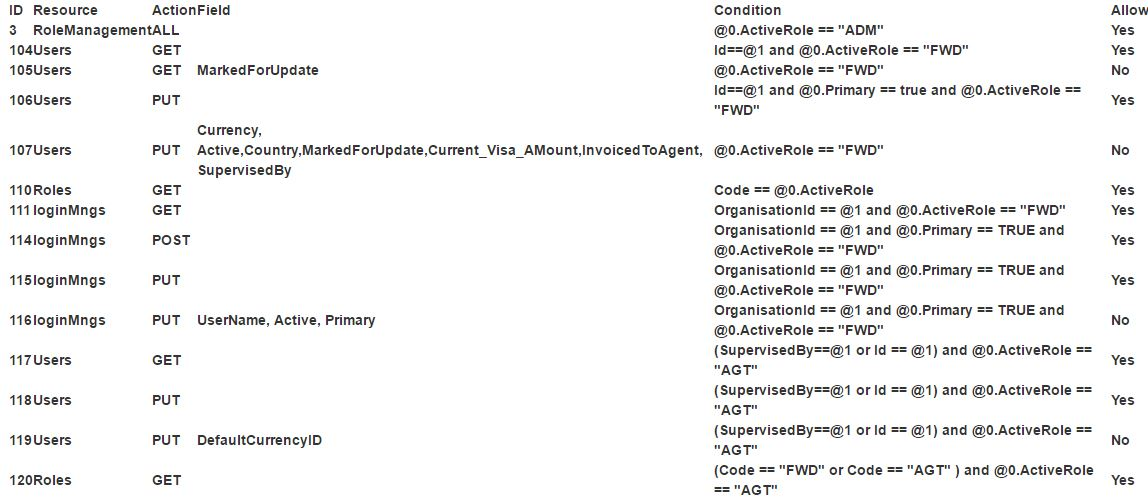
\includegraphics[width=1\textwidth, height=0.24\textwidth]{Img/Tool/ABACPolicies.JPG}
    \caption{Overview policies UI in ABAC}
\end{figure}
\begin{figure}[h]
    \centering
    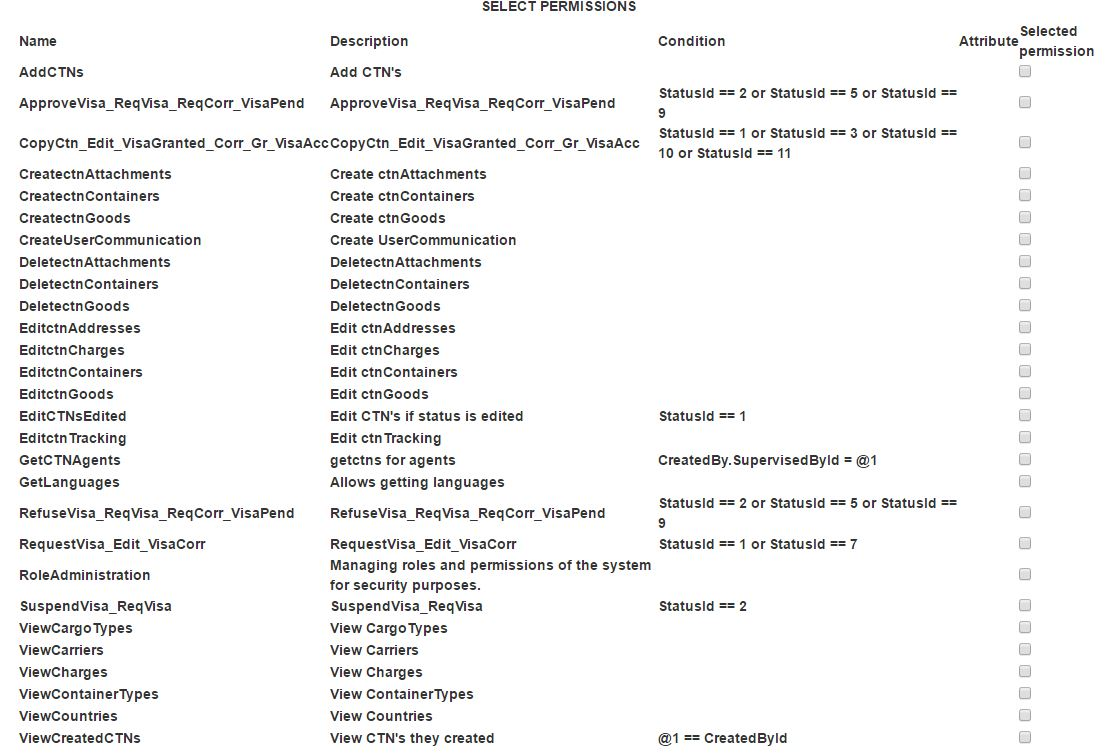
\includegraphics[width=1\textwidth, height=0.24\textwidth]{Img/Tool/RBACPermissions.JPG}
    \caption{Overview permissions UI in AERBAC}
\end{figure}
\\

\textbf{\say{When would you consider the attribute enhanced role based model to be the better choice over the attribute based model? When would you consider using the attribute based model over the attribute enhanced role based model?} }
\\
\\
Users considered the attribute enhanced role based model would perform better than the attribute based model when the system requires the use of many roles, the same was said for systems that have changing requirements, this model was found to be more maintainable.
The attribute based model on the other have was preferred for its quick set up time that the users experienced compared to the attribute enhanced role based model.
It was also preferred when working with systems that do not depend on the use of roles.
\\

\textbf{\say{What is your view on the knowledge that is needed to use the two models effectively? Is there a disparity between the knowledge needed with each model?} }
\\
\\
Both users found that there was no disparity between the two models on the amount of knowledge needed to effectively manage the system.
Both models required a significant amount of knowledge from the user to be used effectively, but since both allow the use of the same type of conditions there is no difference here, apart from conditions being longer with the attribute based model since you need to add in the role check in the conditions.

\textbf{\say{How clear were the interactions between existing policies/permissions and the newly added ones? Was it always clear what the effects of the additions were?} }
\\
\\
The users found that usually it was clear what the effect of adding policies/permissions to the system was, however again due to the interface it was not always clear if the permissions in the attribute enhanced role based system were always assigned correctly to the roles.
One important thing that was pointed out is that you should always keep track of the effects of existing field conditions or adding new ones because these effects can be unclear.
There were however concerns to how this would still be the case when there were many more permissions and policies, but this can be dealt with using filtering.
\\

\textbf{\say{What do you think about the options that are available for constructing conditions?  Would they suffice for the systems you develop? If not what additions could be made?} }
\\
\\
Both users found that the options for making conditions for both systems were sufficient, however it was noted that it would be useful to add negative permissions to the attribute enhanced role based model.
\\

\textbf{\say{Looking at the permissions and policies, how easy to understand is it if you were put there as a new administrator for the system?} }
\\
\\
In its current state it is agreed on that the attribute based model would be clearer for the new admin since that interface contains all the information.
For both models it is also pointed out that the new admin would need significant knowledge of the underlying system, understanding how conditions are made also requires some programming knowledge from the admins and is not fit to be done by non technical personnel.
Using a declarative input language such as XACML\footnote{http://docs.oasis-open.org/xacml/3.0/xacml-3.0-core-spec-os-en.html} would make it more understandable for non technical users.
\\

\textbf{\say{Do you foresee any problems that can arise from using these models in systems that are bigger?} }
\\
\\
The main problems that were foreseen when using the models with a bigger system is that especially with the attribute based model this can gravely impact performance in a negative way.
Concerns were also raised for keeping the oversight of the system but this would not be a big issue for the manageability if we introduce filters and ordering.

\textbf{\say{Are there any features that you think would benefit the different models? What benefits do they provide? Example of possible features: role hierarchy.} }
\\
\\
One user proposed the introduction of negative permissions in the attribute enhanced role based access control model.
We also made a proposal ourselves of adding hierarchical roles to the attribute enhanced role based model, such as discussed in the second chapter.
The users found this to be a good feature to speed up using the model in question, for the attribute based model this extension is not so straight forward since there is no link between roles and policies outside of the conditions.
\\

\textbf{\say{Looking at it as a developer, which model would be best to make the users easily understand their access rights? Why do you think this is the case?} }
\\
\\
The attribute enhanced role based model was considered to be the easiest to develop a visualization for that made it clear for users of the system which rights they had.
This can be attributed to the permissions being linked to the roles, we would not have to make a full evaluation of all the policies available in the system for that object, which would have to be done for the attribute based model.

\subsection{Overall conclusion}
In first instance looking at the results it becomes clear the users generally preferred the attribute based model. 
A lot of that preference had to do with the user interface and how this was setup as has been pointed out by the users.
When looking deeper into this we conclude that if more time is put into a better user interface this will greatly improve the manageability of the attribute enhanced role based model, for the attribute based model there is little improvement to be had using more than the basic interface.
When we only have this basic interface the attribute based model is considered to be the better model on the level of manageability, when we create a more expansive user interface the attribute enhanced role based model will be more manageable. 
\\
\\
On the level of extensibility and understandability the preference goes out to the attribute enhanced role based model.
The link with the permissions and roles makes it easier to visualize to users of the system what they are allowed to do.
This model is also the most extensible model of the two, allowing for easier adaptation.
For maintainability the attribute enhanced role based model was also the one preferred since it did not require many changes to permissions if a new role is added to the system or the requirements change.

\section{Results performance}

\subsubsection{Data}
This data is the average of 100 calls to the system under each of the models, we have the baseline model which is the existing implementation, the attribute enhanced role based model (AERBAC) and the attribute based model (ABAC).
We accessed the system with 3 different users FWD, AGT and ADM.
We have provided the full raw data represented in charts in below, except for the baseline.

\begin{table}[ht]
    \begin{tabular}{ |p{3cm}|p{3cm}|p{3cm}|p{3cm}|  }
        \hline
        \multicolumn{4}{|c|}{Average response time performance} \\
        \hline
        Model & FWD & AGT & ADM\\
        \hline
        Baseline & 0.135 sec   & 0.110 sec   & 0.101 sec  \\
        AERBAC & 0.268 sec    & 9.508 sec    & 0.088 sec  \\
        ABAC & 28.394 sec   & 9.923 sec    & 8.189 sec    \\
        \hline
    \end{tabular}
    \caption{Table results performance}
\end{table}

\begin{figure}[h]
    \centering
    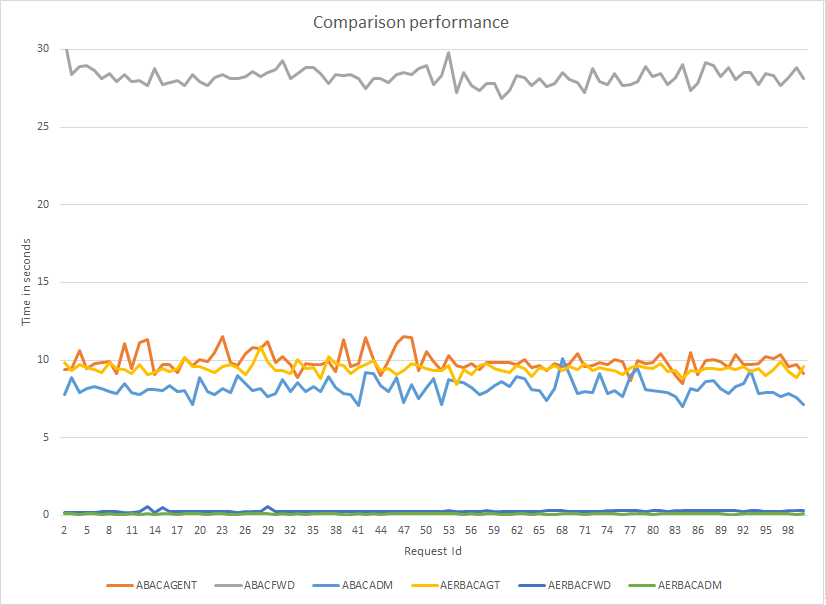
\includegraphics[width=0.9\textwidth, height=0.6\textwidth]{Img/Performance/Perf.png}
    \caption{Comparison implemented models normal scale}
\end{figure}
\begin{figure}[h]
    \centering
    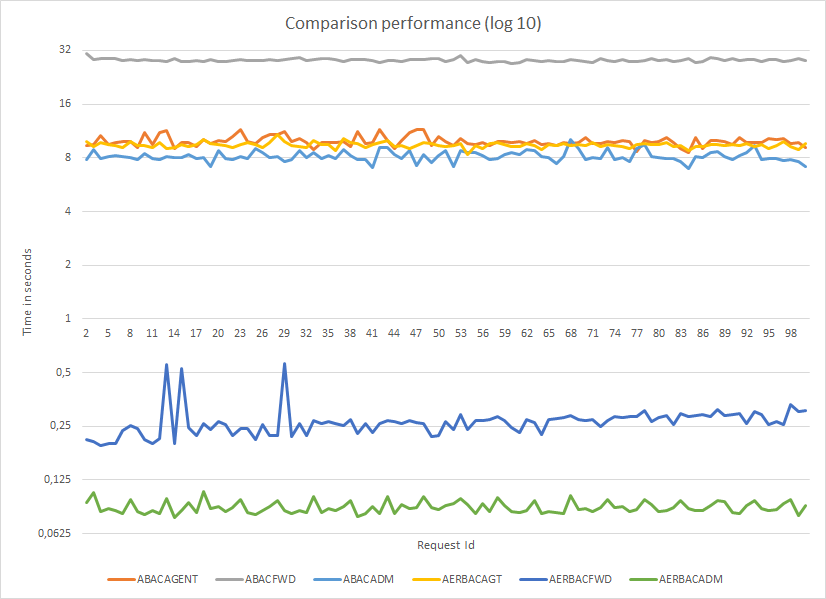
\includegraphics[width=0.9\textwidth, height=0.6\textwidth]{Img/Performance/PerfLog10.png}
    \caption{Comparison implemented models logarithmic scale}
\end{figure}

\subsubsection{Conclusion}
When analyzing this data it becomes clear rather quickly that there are some issues here.
We can see that with the attribute enhanced role based model we still have a performance within the order of magnitude of the base line, in case of the ADM role even better.
However for the agent role we immediately see a performance that is a lot worse.
This issue becomes even more dramatic when we look at the attribute based model.
\\
\\
After searching for where the problem lies it becomes clear that dynamic linq is not mature enough to cope with more complex conditions.
When using conditions that require joins, such as is needed for the AGT role, it does not translate everything to queries which leads to loading all the data in memory.
Further analysis and reasoning between the models can still be done but we need to keep in mind this problem on the implementation level.
\\
\\
One of the first things we notice is that for the attribute enhanced role based model neither the ADM and FWD roles are impacted by this problem.
The reason for this is that the conditions placed are very minimal for both of these roles, they are simple non-combined conditions that do not require any joining of tables.
Looking at these we can also see that the ADM role is still significantly faster than the FWD role.
This is to be attributed to the ADM role having fewer permissions that are assigned to it, while the FWD role has more permissions that are assigned to it for the objects being requested.
This lets us conclude that there is a meaningful impact of the evaluation of the number of permissions assigned to roles on the performance of the models.
This also lets us conclude that the impact on the performance compared to the baseline can be limited and does not pose an issue on the tested scale, given that the problem of the evaluation component can be mitigated.
\\
\\
A second observation is that when using the attribute based model all roles are affected by the problem in the evaluation component.
This while the ADM role especially does not have more conditions or more difficult conditions than with the attribute enhanced role based model.
We see that is is also affected by the problems that manifest themselves with the policies aimed at the AGT role, this is due to the nature the attribute based model works.
Out of this we can conclude that the attribute based model will be slower since it has to evaluate every policy on the object type for every role.
Even if that policy says it is for a different role and lazy evaluation is used, where  we stop evaluating conditions when the result cannot change by any conditions that follow in combination with and/or operators, we still have to do the joins to start evaluating.
Another result is that contrary to the attribute enhanced role based model the FWD role has an even more dramatic performance than the AGT role.
This can be explained due to the complexity of the conditions that  increased using this model.
When actually evaluating the roles lazy evaluation leads to stopping the evaluation of the condition once the first part returns false (comparing the roles).
This prevented more complex and longer condition of being executed for the other roles, but this still impacted the FWD role for which they were meant heavily.
\\
\\
There is one big conclusion that can be made on the level of performance, even with the issues there exists with the evaluation component.
The conclusions being that with the attribute based model we need to evaluate a lot more conditions, with the attribute enhanced role based model on the other hand we first have get the role and extract the permissions assigned to this role and then evaluate the conditions for that role only.
The evaluation of conditions is the more performance intensive operation of the two, which leads to a preference for the attribute enhanced role based model on the level of performance.
However making more conclusions with the current implementation are hard  and difficult to justify.

\chapter{Conclusions}
\label{chapt:Conclusions}
Out of the experiment we have done multiple conclusions can be made, some in preference of the attribute based model and others in preference of the attribute enhanced role based model.
First of all we can conclude that the role based access control model does not suffice if we need a more fine grained solution to access control.
This can however be resolved by using combined models such as the attribute enhanced role based access control model.
We can also conclude that the attribute based model is more user friendly when using a very basic user interface, if we spend more time on the interface however the users of the system see the attribute enhanced role based model to benefit most and become easier to use.
When we compared the two models with each other we came to the conclusion that the attribute based model allowed users the set up the system faster than the attribute enhanced role based model.
The flip side of this is that the attribute based model is more error sensitive, where a mistake in any rule can cause problems for every access attempt of those objects, this is not the case for the attribute enhanced role based model.
On the level of maintainability the users concluded that when the requirements changed the attribute enhanced role based model is more robust to these changes and easiest to adapt to these changes.
The users found the attribute enhanced role based model to be the most straightforward model to use as a developer to make it clear for the other users of the system what their rights are within the system.
Performance wise we conclude that much of the performance depends on the rules that have to be evaluated by the system with each access attempt.
Generally this number is lower when using the attribute enhanced role based model with permissions while the attribute based model with policies requires more policies to be checked, leading to poorer performance.

\section{Related work}
There are a wide variety of studies that have been conducted to compare different access control models in different circumstances and environments.
Sonu Verma et al have done a comparison of role based access control and attribute based access control in semantic web in Comparative analysis of Role Base and Attribute Base Access Control Model in Semantic Web \cite{Related1}.
This study showed how role based access control itself is not as fine grained as attribute based access control which is why we also took a different model.
Shabnam Mohammad Hasani et al have done an extensive study in Criteria Specifications for the Comparison and
Evaluation of Access Control Models on how we can compare the different access control models \cite{Related3} from which we also used criteria in our study.
In Mohammed ENNAHBAOUI et al. their work Study of Access Control Models \cite{Related2} a comparison between the higher level models is done, mandatory access control, discretionary access control, role based access control and organizational based access control.



\section{Future work}
A lot of future work can still be done on the subject, we have only done a comparison between two models but we can compare these with the other models mentioned in chapter two.
An expansion can be made that compares the chosen models with the task role based access control since this model also meets the requirements set up by the tested system.
Other future work lies in creating more new models by combination of the features of both role based access control and attribute based access control.
We used one such combination in this study but many more can be made, as explained by Timothy R Weil et al in Adding attributes to role based access control \cite{Combined1}.
They should first be worked out theoretically since not much has been done on that subject, we mentioned two of the existing models in chapter two.
This can be in conjunction with a case study.
\backpages

%%%%%%%%%%%%%%%%%%%%%%%%%%%%%%%%%%%%%%%%%%%%%%%%%%%%%%%%%%%%%%%%%%%
\begin{appendices}
\chapter{Scenario's}
\label{appendix:scenario}
This appendix describes the scenarios we used to test correctness and that the users had to perform as part of studying manageability.
These 2 scenario's are based on an existing application.

\section{Scenario 1}
This scenario has 3 different roles which all have certain privileges to view (get), create (post) or edit (put) different resources. There are also actions that can only be done by a certain role. 
\\
The roles have to be created with the corresponding 3 letter code behind them. A user should be assigned to each role. In case of the admin role (ADM) this is already done since this is a prerequisite to use the system.

\subsection{Forwarder(FWD)}
\begin{itemize}
    \item Can only view the CTN's they created.
    \item Can add CTNs to the system.
    \item Can edit CTN's if status is edited.
    \item Can view all off the following data: CargoTypes, IncoTerms, Carriers, Currencies, Countries, CTNCities, FreightPaymentTypes, ctnAddresses, ctnTracking, ctnAttachments, ctnCharges, ctnGoods, ctnContainers, TransportTypes, UserCommunication, GoodsClassifications, ContainerTypes, Statuses, Charges, IMOs, Locations.
    \item Can Create all of the following data: UserCommunication, ctnGoods, ctnContainers, ctnAttachments.
    \item Can delete following data: ctnAttachments, ctnContainers, ctnGoods.
    \item Can edit all of the following data: ctnTracking, ctnCharges, ctnAddresses, ctnGoods, ctnContainers. 
    \item Can perform action requestvisa if ctn status is edited or visa corrected.
    \item Can perform action copyctn if ctn status is edited, visa granted, correction granted, visa accepted.
    \item The user SEAFRIGO should be assigned to this role.
\end{itemize}

\subsection{Agent(AGT)}
\begin{itemize}
    \item Can view all the CTN's associated with forwarders they manage.
    \item Can view all off the following data: ctnAddresses, ctnTracking, ctnAttachments, ctnCharges, ctnGoods, ctnContainers, UserCommunication.
    \item Can Create all of the following data: UserCommunication.
    \item Can perform action approvevisa if ctn status is Requested visa, requested correction or visa pending.
     \item Can perform action refusevisa if ctn status is Requested visa, requested correction or visa pending.
     \item Can perform action suspendvisa if ctn status is Requested visa.
     \item The user AGENTFRANCE should be assigned to this role.
\end{itemize}

\subsection{Admin(ADM)}
\begin{itemize}
    \item Can view all the CTN's.
    \item Can view all off the following data: ctnAddresses, ctnTracking, ctnAttachments, ctnCharges, ctnGoods, ctnContainers, UserCommunication.
     \item Can Create all of the following data: UserCommunication.    
\end{itemize}

\section{Scenario 2}
This scenario also has 3 different roles which all have certain privileges to view (get), create (post) or edit (put) different resources.
There are also actions that can only be done by a certain role.
Some values have to be hidden so they cannot be seen or cannot be edited.
\\
The roles have to be created with the corresponding 3 letter code behind them. A user should be assigned to each role. In case of the admin role (ADM) this is already done since this is a prerequisite to use the system.

\subsection{Forwarder(FWD)}
\begin{itemize}
    \item Can only see their own User object,  cannot view the fields MarkedForUpdate and Current\_Visa\_Amount.
    \item Can edit User object if it is their own User and the login is the primary login for this User. Cannot edit role, currency, active, country, MarkedForUpdate, Current\_Visa\_Amount, InvoicedToAgent or SupervisedBy.
    \item Can view all languages, countries and currencies.
    \item Can only view its own role.
    \item Can only view LoginMngs associated with their User object.
    \item Can add LoginMngs if they belong to the User object and they are the primary login.
    \item Can edit LoginMngs where OrganisationId is the same as their User and they are the primary login, cannot edit the username, active and primary fields.
    \item The user SEAFRIGO should be assigned to this role.
\end{itemize}

\subsection{Agent(AGT)}
\begin{itemize}
    \item Can view user objects that are supervised by this agent and its own associated user.
    \item Can view user objects that are supervised by this agent and its own associated user but cannot edit the DefaultCurrencyId.
    \item Can view roles with code FWD or EXP.
    \item Can view all languages, countries and currencies.
    \item Can view all LoginMngs of user objects they supervise.
    \item Can add LoginMngs of user objects they supervise.
    \item Can edit LoginMngs of user objects they supervise, cannot edit the username, active and primary fields.
    \item The user AGENTFRANCE should be assigned to this role.
\end{itemize}

\subsection{Admin(ADM)}
\begin{itemize}
    \item Can view all user objects.
    \item Can edit all user objects except for their DefaultCurrencyId.
    \item Can view all roles.
    \item Can view all languages, countries and currencies.
    \item Can view all LoginMngs.
    \item Can add LoginMngs.
    \item Can edit LoginMngs, cannot edit the username, active and primary fields.
\end{itemize}
\chapter{Interview}
\label{appendix:interview}

This appendix contains the questions that were asked to the participants of our experiment.
This interview is mainly for evaluating the positives and negatives of the different models from the side of the users and people that will manage and/or develop these systems.
This as goal to get qualitative on the different models.
The interview takes around 30 minutes and we have written down and recorded the answers given by the participants.

\section{Factual questions}

\begin{enumerate}
    \item Different models have been tested, can you tell us which features you used and were needed to complete the different scenario's? which actions had to be done to complete these scenario's?
    
    \item Were you able to complete all requested actions in the scenario, given the available feature set? Which tasks went well?
   
    \item When using conditions did you prefer adding 1 permission/policy with complex conditions or multiple permissions/policies with simple conditions?
    
\end{enumerate}

\clearpage

\section{Opinion questions}

\begin{enumerate}
    \item Which model did you prefer using for management in the different scenario's?
    
    \item When would you consider the attribute enhanced role based model to be the better choice over the attribute based model? When would you consider using the attribute based model over the attribute enhanced role based model?
    
    \item What is your view on the knowledge that is needed to use the 2 models effectively? Is there a disparity between the knowledge needed with each model?
    
    \item How clear were the interactions between existing policies/permissions and the newly added ones? Was it always clear what the effects of the additions were?
    
    \item What do you think about the options that are available for constructing conditions?  Would they suffice for the systems you develop? If not what additions could be made?
    
    \item Looking at the permissions and policies, how easy to understand would it be if you were put there as a new administrator for the system?
    
    \item Do you foresee any problems that can arise from using these models in systems that are bigger?
    
    \item Are there any features that you think would benefit the different models? What benefits do they provide? Example of possible features: role hierarchy.
    
    \item Looking at it as a developer, which model would be best to make the users easily understand their access rights? Why do you think this is the case?
    
\end{enumerate}


%\chapter{Performance}
\label{appendix:performance}

\section{Default system}
\subsection{FWD}
\csvautolongtable{Performance/CCCBesc2SEAFRIGO100.txt}
\subsection{AGT}
\csvautolongtable{Performance/CCCBesc2AGENTFRANCE100.txt}
\subsection{ADM}
\csvautolongtable{Performance/CCCBesc2TC&T100.txt}

\section{Attribute enhanced role based system}
\subsection{FWD}
\csvautolongtable{Performance/CCCBesc2_RBACSEAFRIGO100.txt}
\subsection{AGT}
\csvautolongtable{Performance/CCCBesc2_RBACAGENTFRANCE100.txt}
\subsection{ADM}
\csvautolongtable{Performance/CCCBesc2_RBACTC&T100.txt}

\section{Attribute based system}
\subsection{FWD}
\csvautolongtable{Performance/CCCBesc2_ABACSEAFRIGO100.txt}
\subsection{AGT}
\csvautolongtable{Performance/CCCBesc2_ABACAGENTFRANCE100.txt}
\subsection{ADM}
\csvautolongtable{Performance/CCCBesc2_ABACTC&T100.txt}


\end{appendices}

%%%%%%%%%%%%%%%%%%%%%%%%%%%%%%%%%%%%%%%%%%%%%%%%%%%%%%%%%%%%%%%%%%%
\end{document}
